\section{Modelo de implementación según la tecnología elegida}

\subsection{Modelo lógico relacional}

El modelo lógico conserva las tres áreas conceptuales. Las tablas, columnas,
claves y relaciones se reparten entre tres figuras. Las
Figuras~\ref{fig:logico-operacion} a~\ref{fig:logico-interaccion} deben leerse
en conjunto.

\begin{landscape}
\begin{figure}[p]
\centering
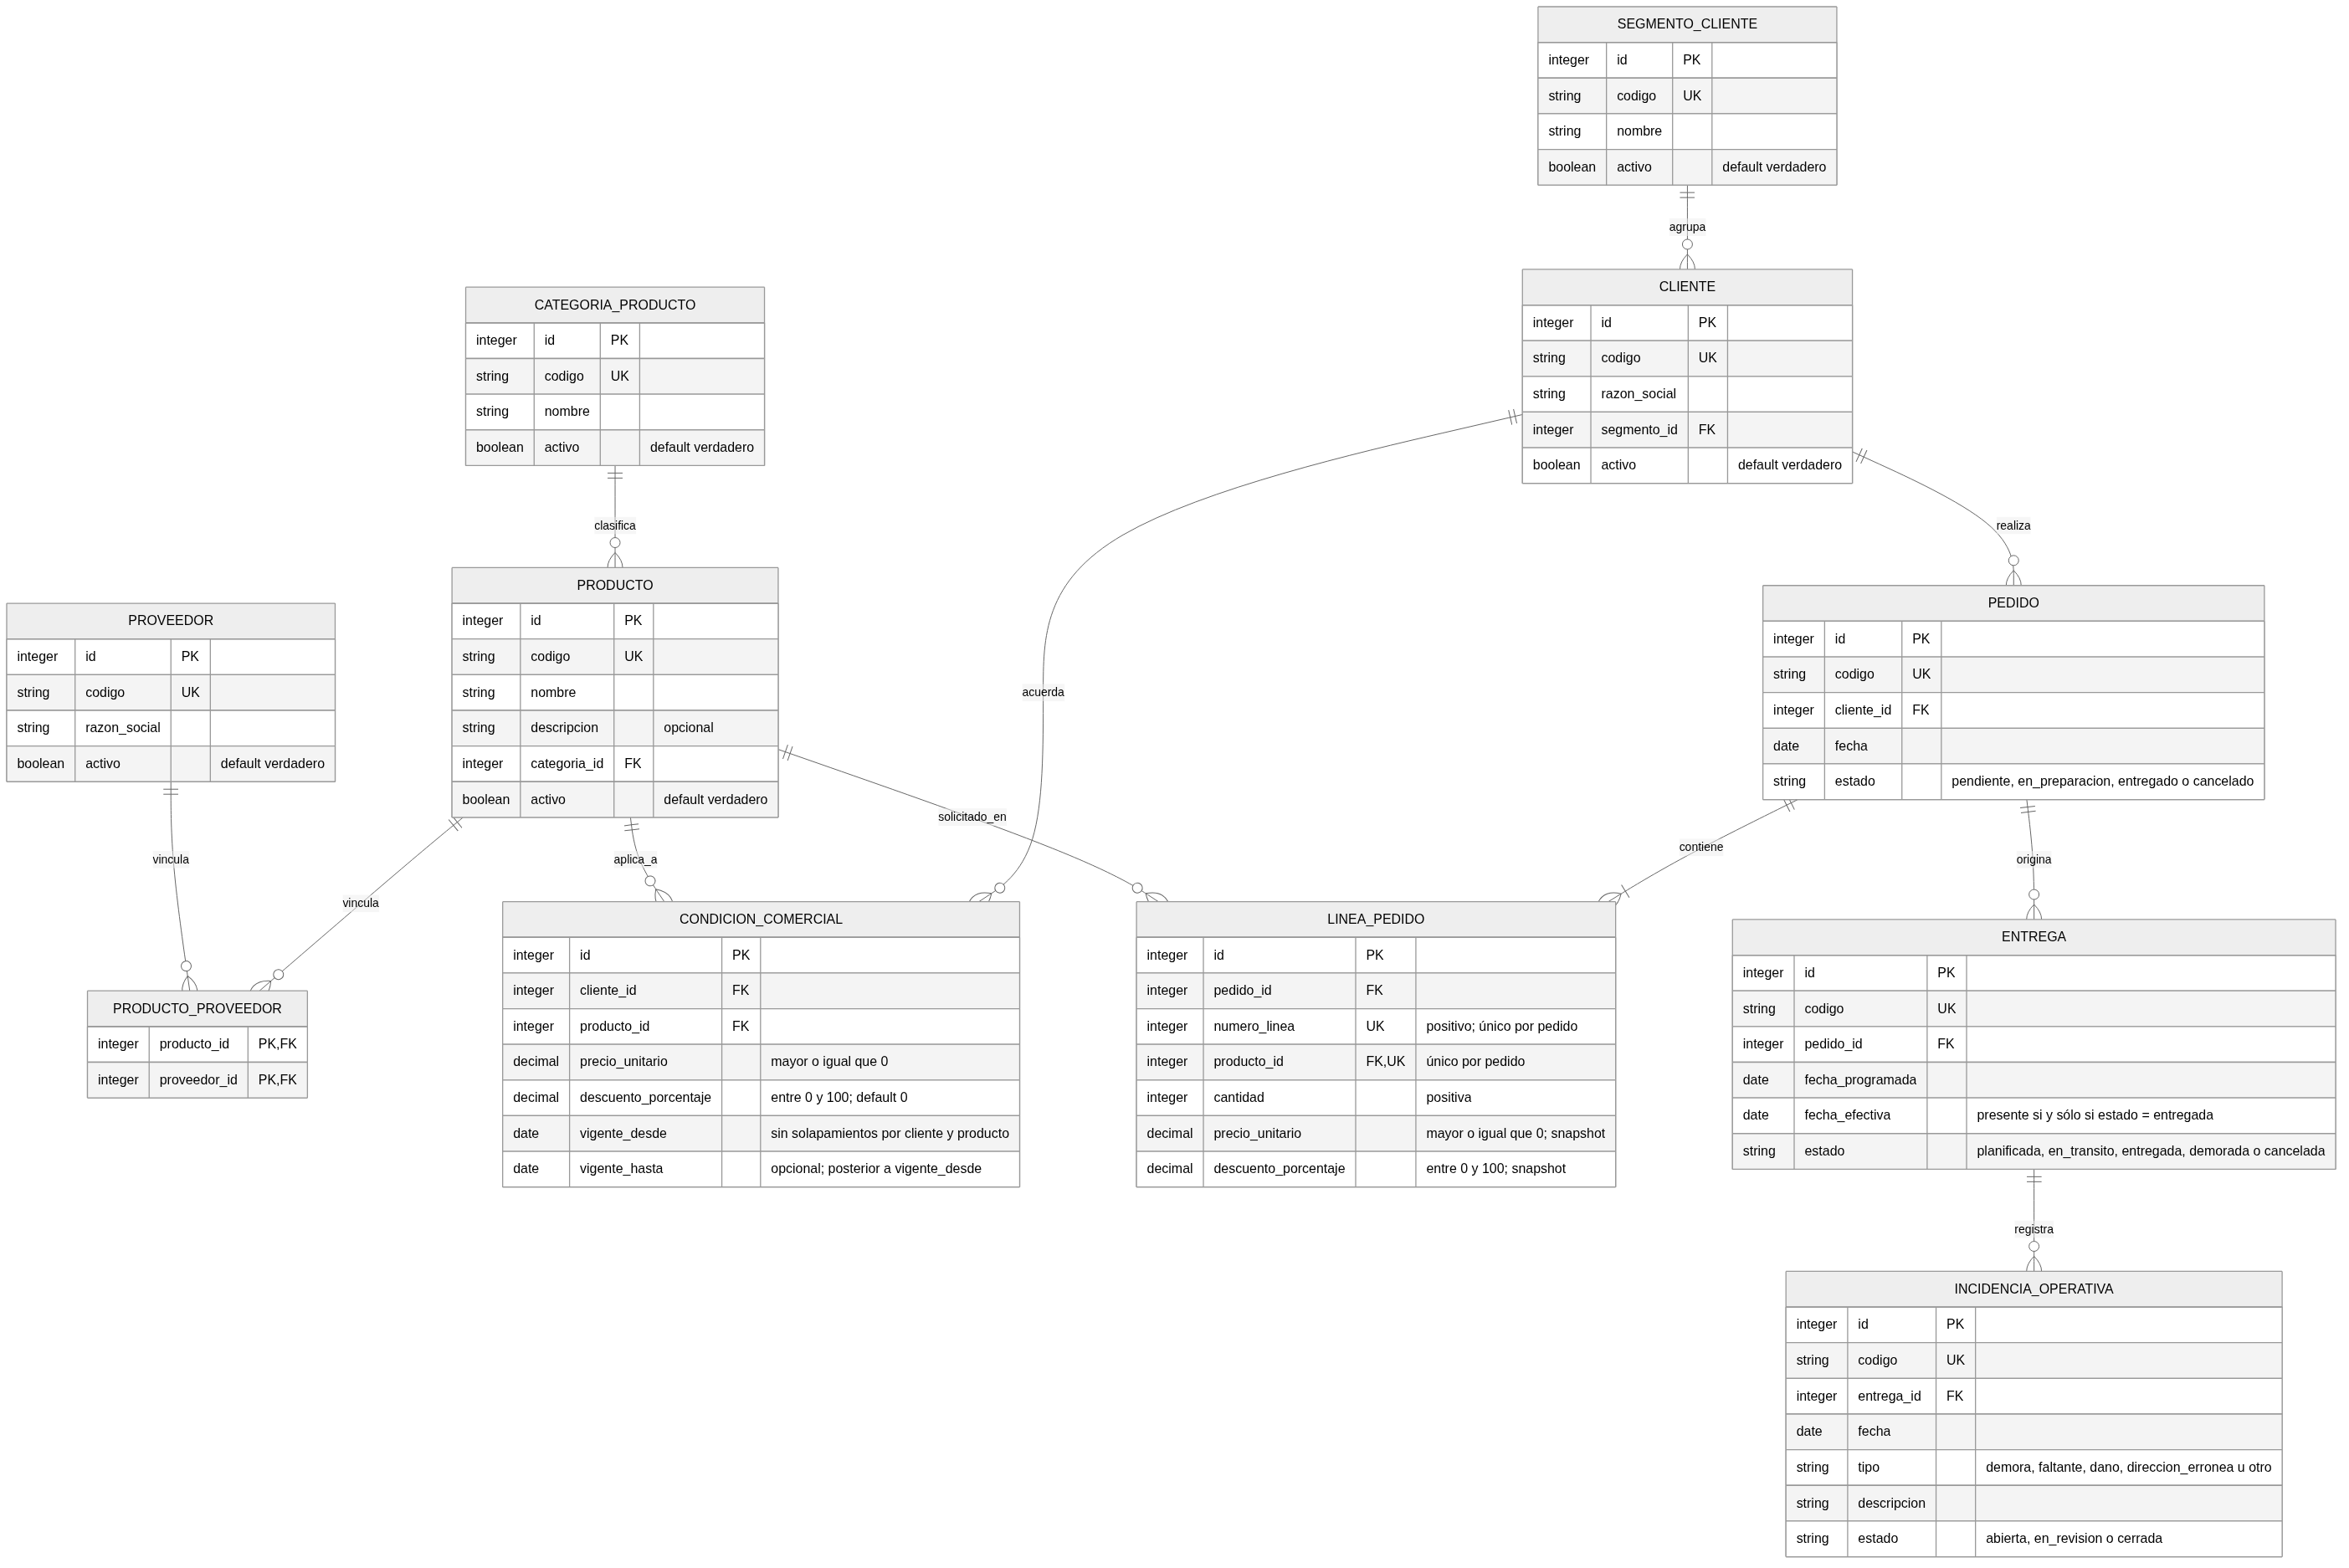
\includegraphics[width=0.85\linewidth]{logico_operacion.png}
\caption{Modelo lógico de la operación comercial y logística.}
\label{fig:logico-operacion}
\end{figure}
\end{landscape}

\begin{figure}[htbp]
\centering
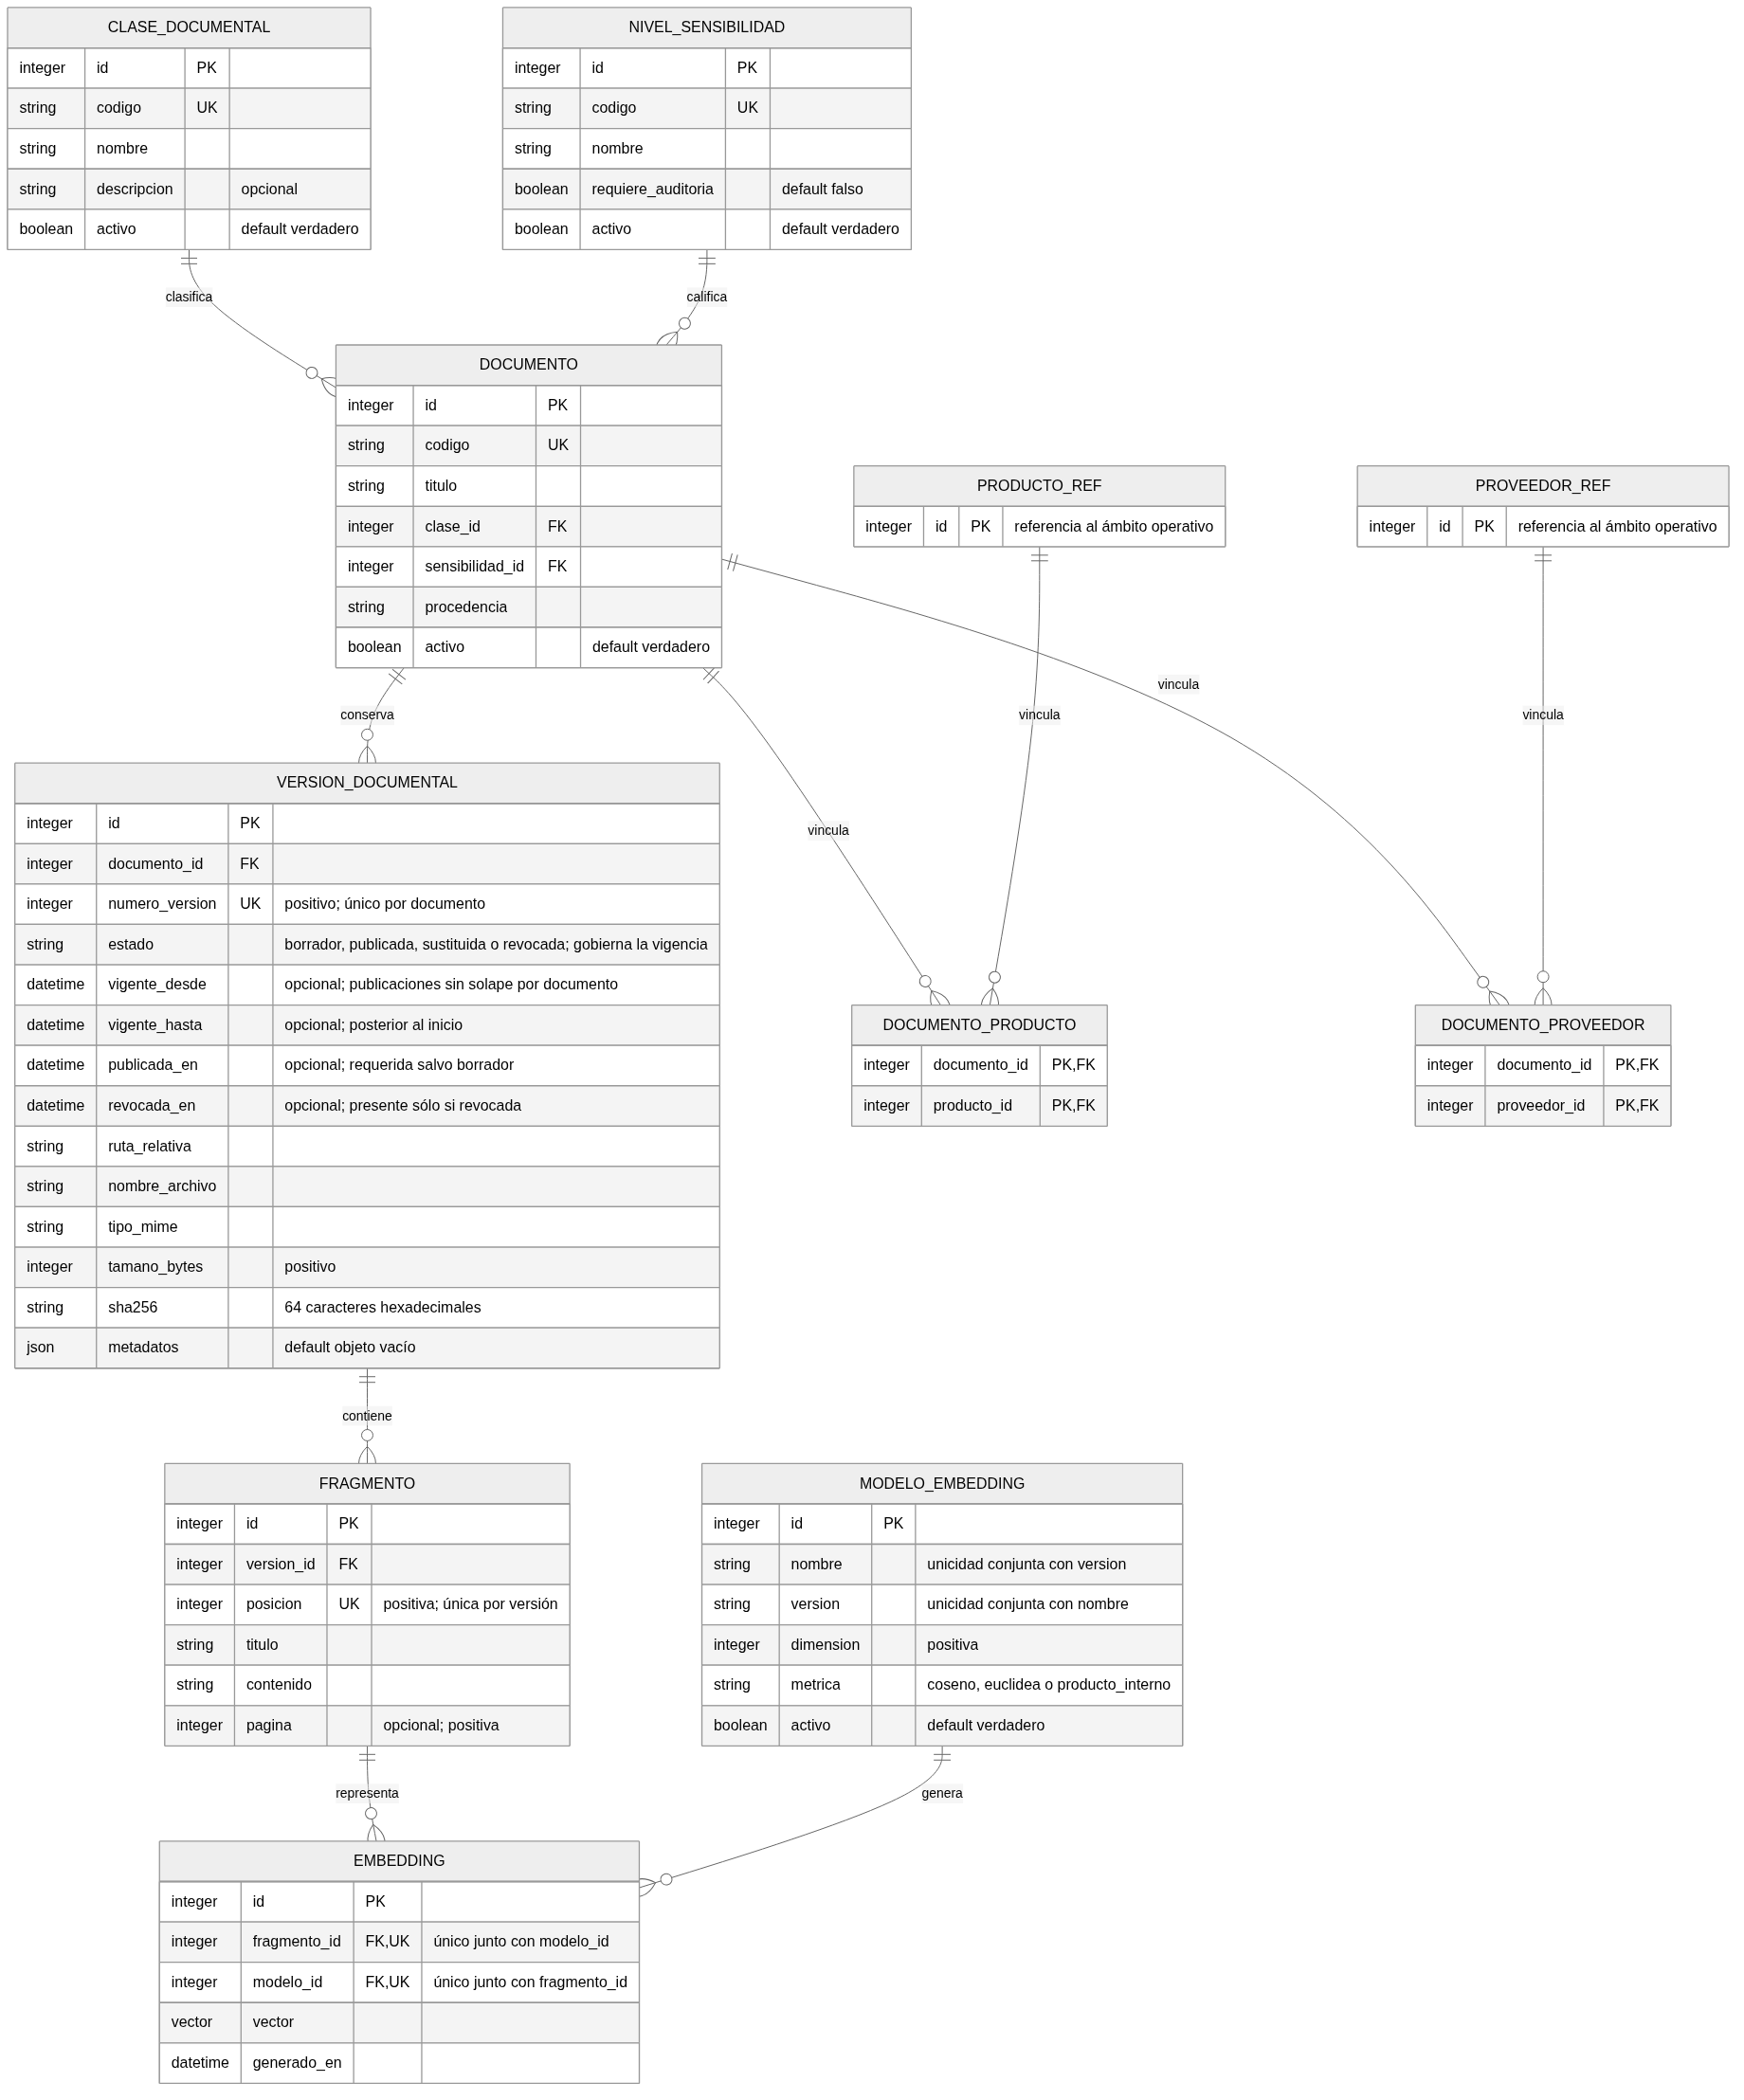
\includegraphics[width=\textwidth]{logico_documentos_recuperacion.png}
\caption{Modelo lógico de documentos y recuperación.}
\label{fig:logico-documentos}
\end{figure}

\begin{landscape}
\begin{figure}[p]
\centering
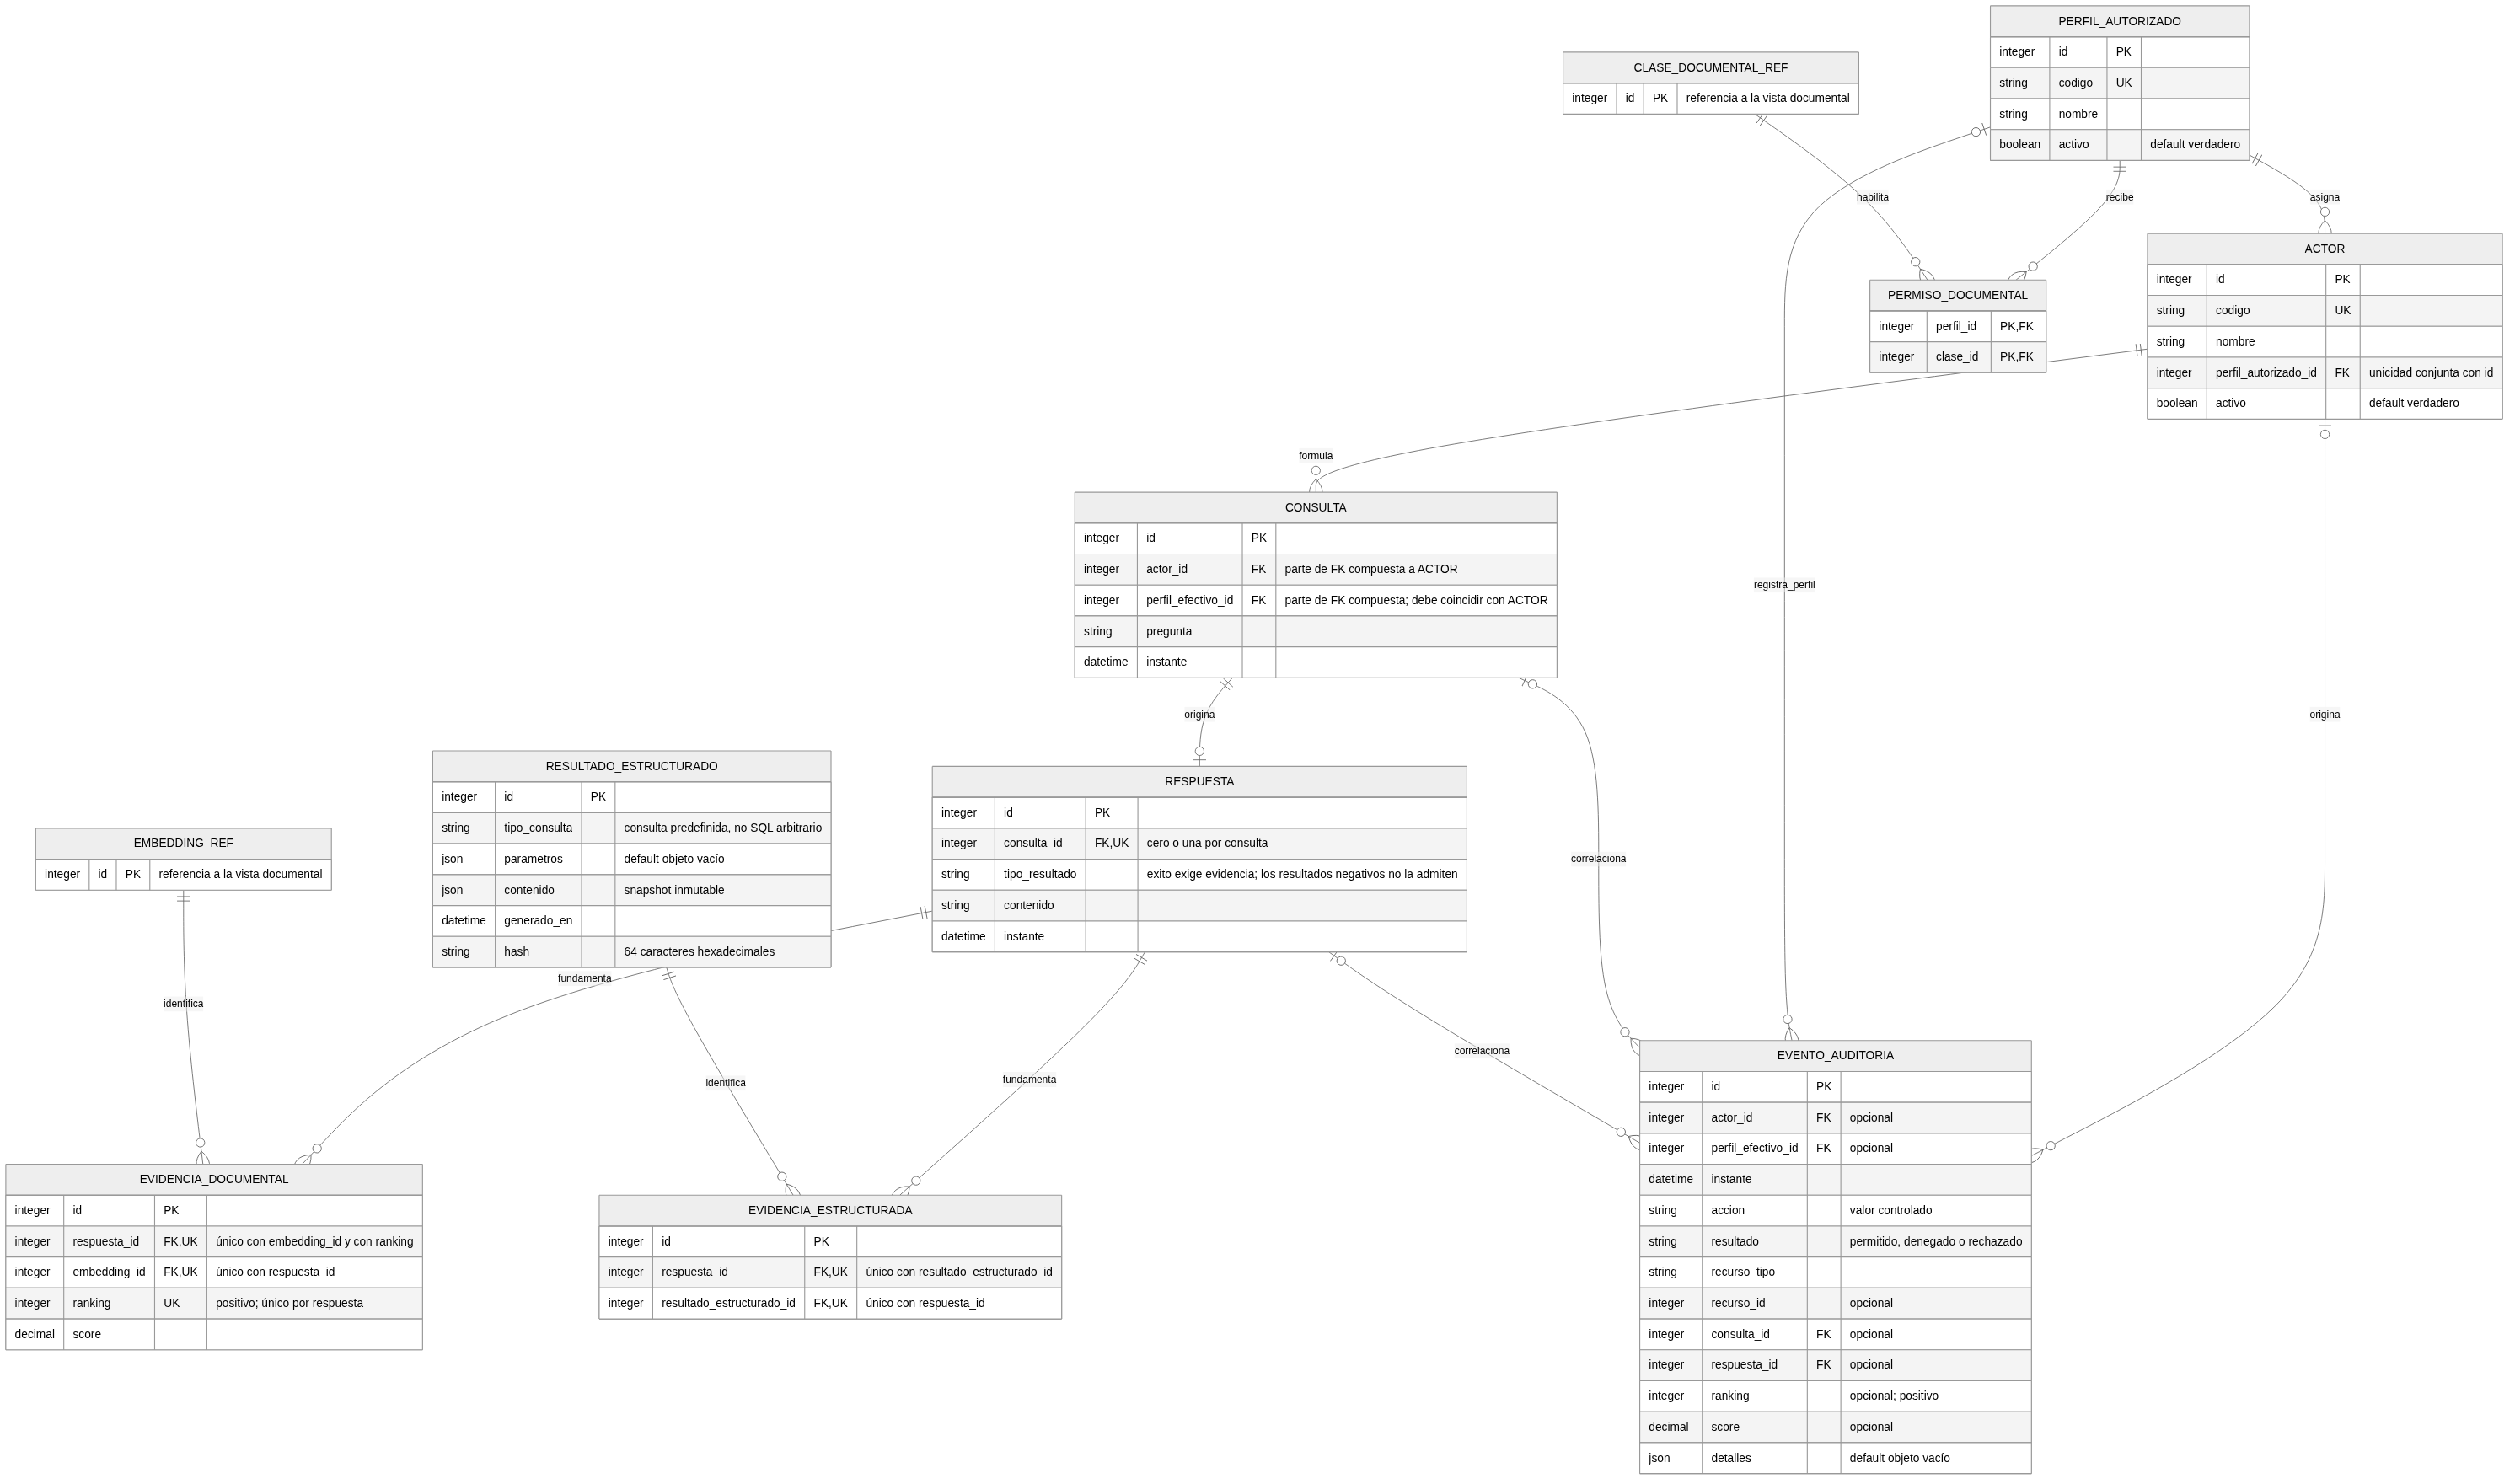
\includegraphics[width=0.85\linewidth]{logico_acceso_interaccion_evidencia.png}
\caption{Modelo lógico de acceso, interacción y evidencia.}
\label{fig:logico-interaccion}
\end{figure}
\end{landscape}
\FloatBarrier

Las entidades con identidad propia usan claves sustitutas. Los códigos de
producto, cliente, proveedor, pedido y documento son claves de negocio únicas.
Las tablas asociativas usan claves compuestas cuando dos referencias identifican
la fila. El recorrido documental enlaza
\texttt{documento}, \texttt{version\_documental}, \texttt{fragmento} y
\texttt{embedding}. La evidencia conserva la referencia exacta de la fuente.
\FloatBarrier

\subsection{Modelo físico en PostgreSQL}

El modelo físico lleva el diseño a PostgreSQL. Las
Figuras~\ref{fig:fisico-operacion} a~\ref{fig:fisico-seguridad} muestran las
tablas, los tipos y las restricciones de cada área. Los scripts de \path{db/}
definen el comportamiento implementado.

\begin{landscape}
\begin{figure}[p]
\centering
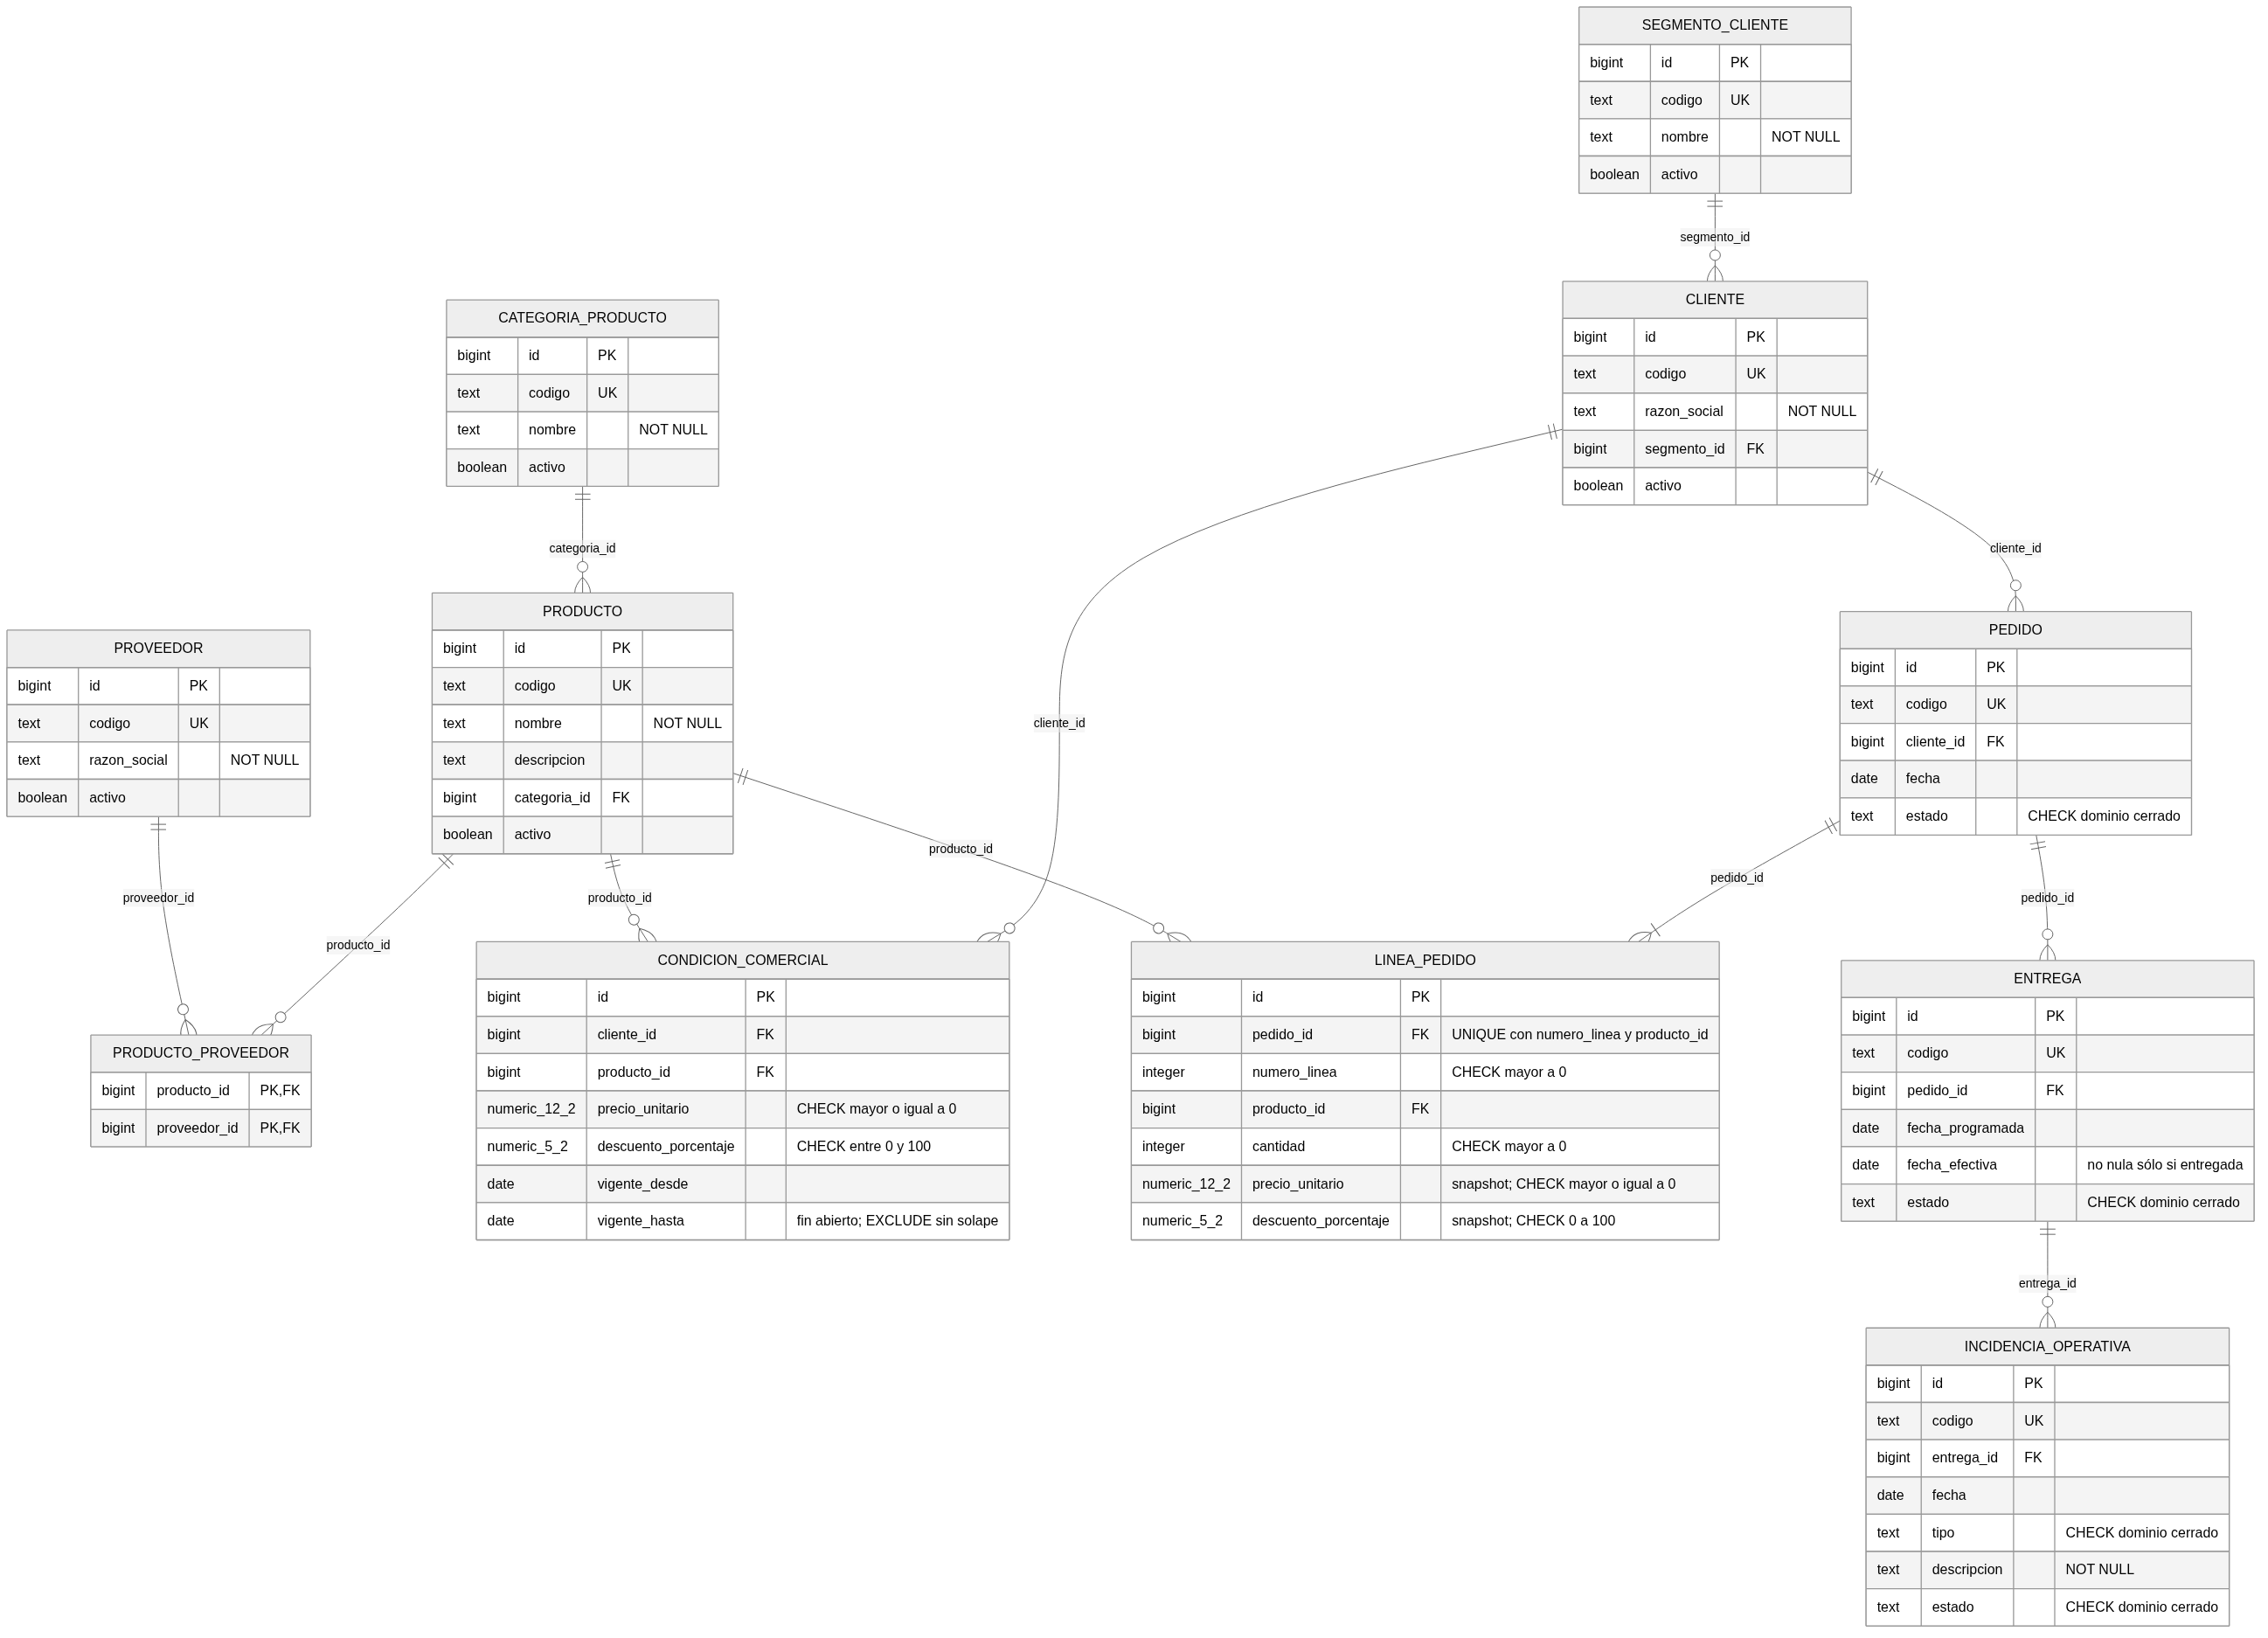
\includegraphics[width=0.82\linewidth]{fisico_operacion.png}
\caption{Implementación física de la operación comercial y logística.}
\label{fig:fisico-operacion}
\end{figure}
\end{landscape}

\begin{figure}[htbp]
\centering
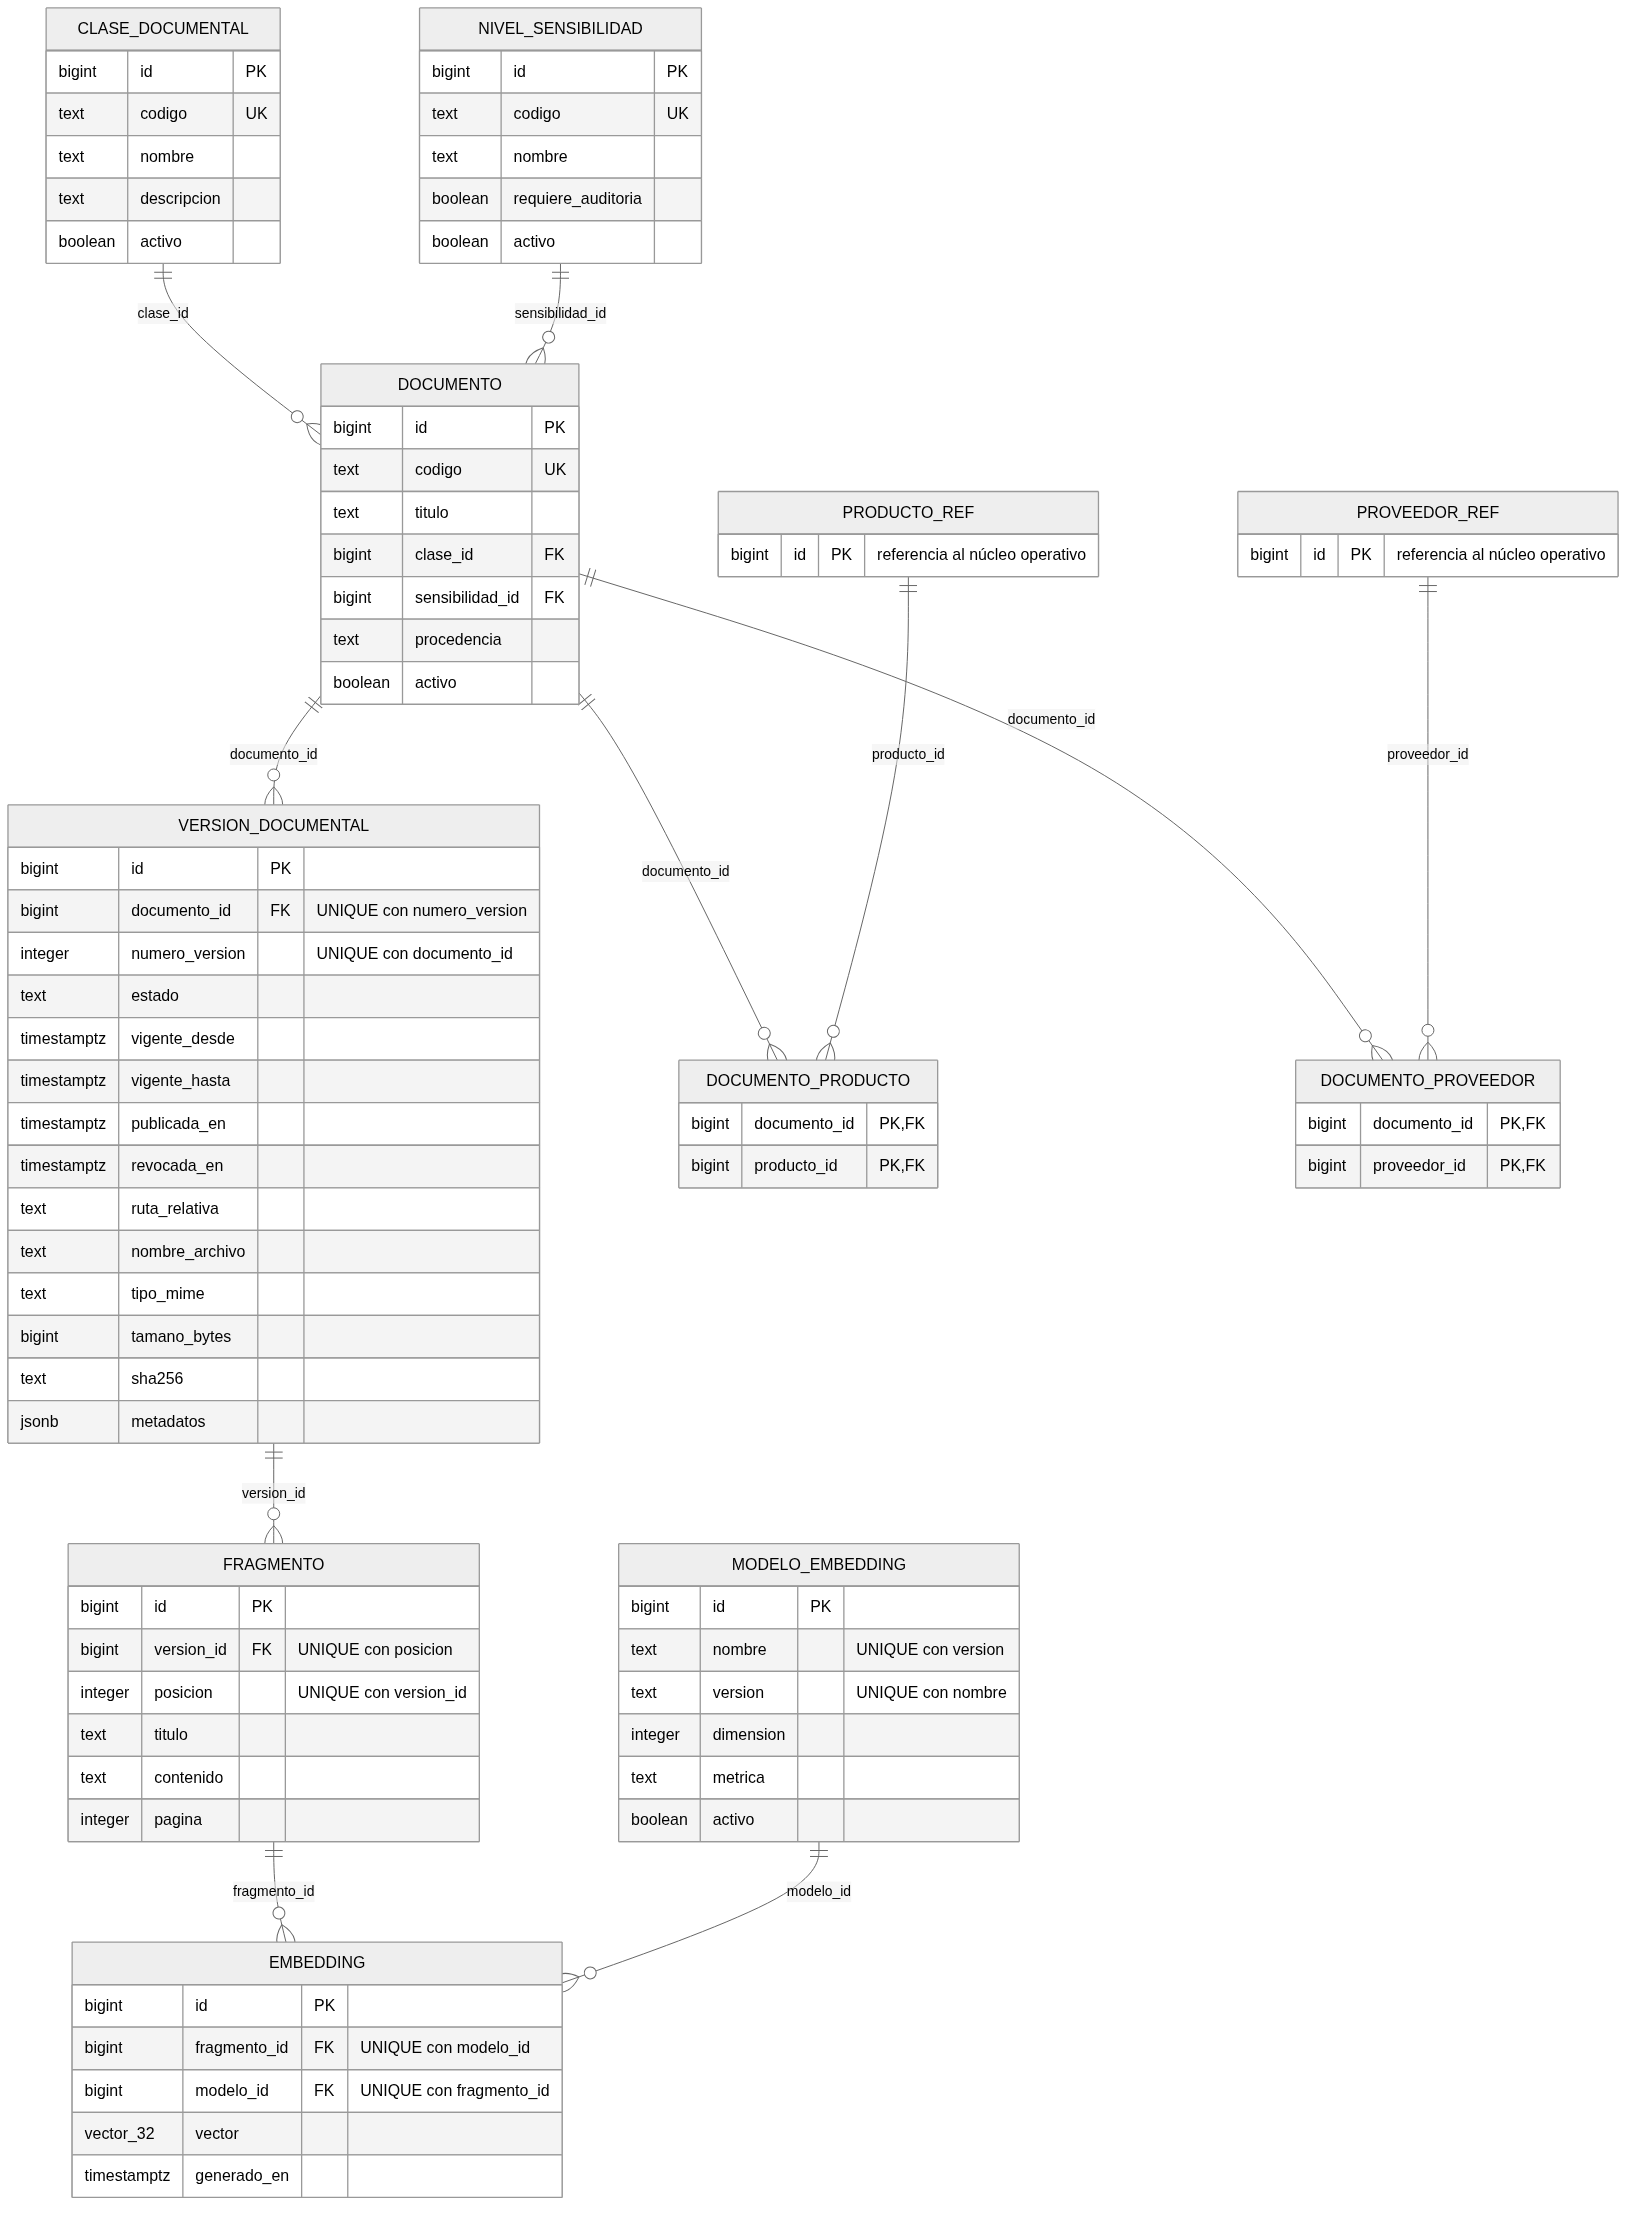
\includegraphics[width=\textwidth,height=0.78\textheight,keepaspectratio]{fisico_recuperacion.png}
\caption{Almacenamiento, vigencia y recuperación vectorial en PostgreSQL.}
\label{fig:fisico-recuperacion}
\end{figure}

\begin{landscape}
\begin{figure}[p]
\centering
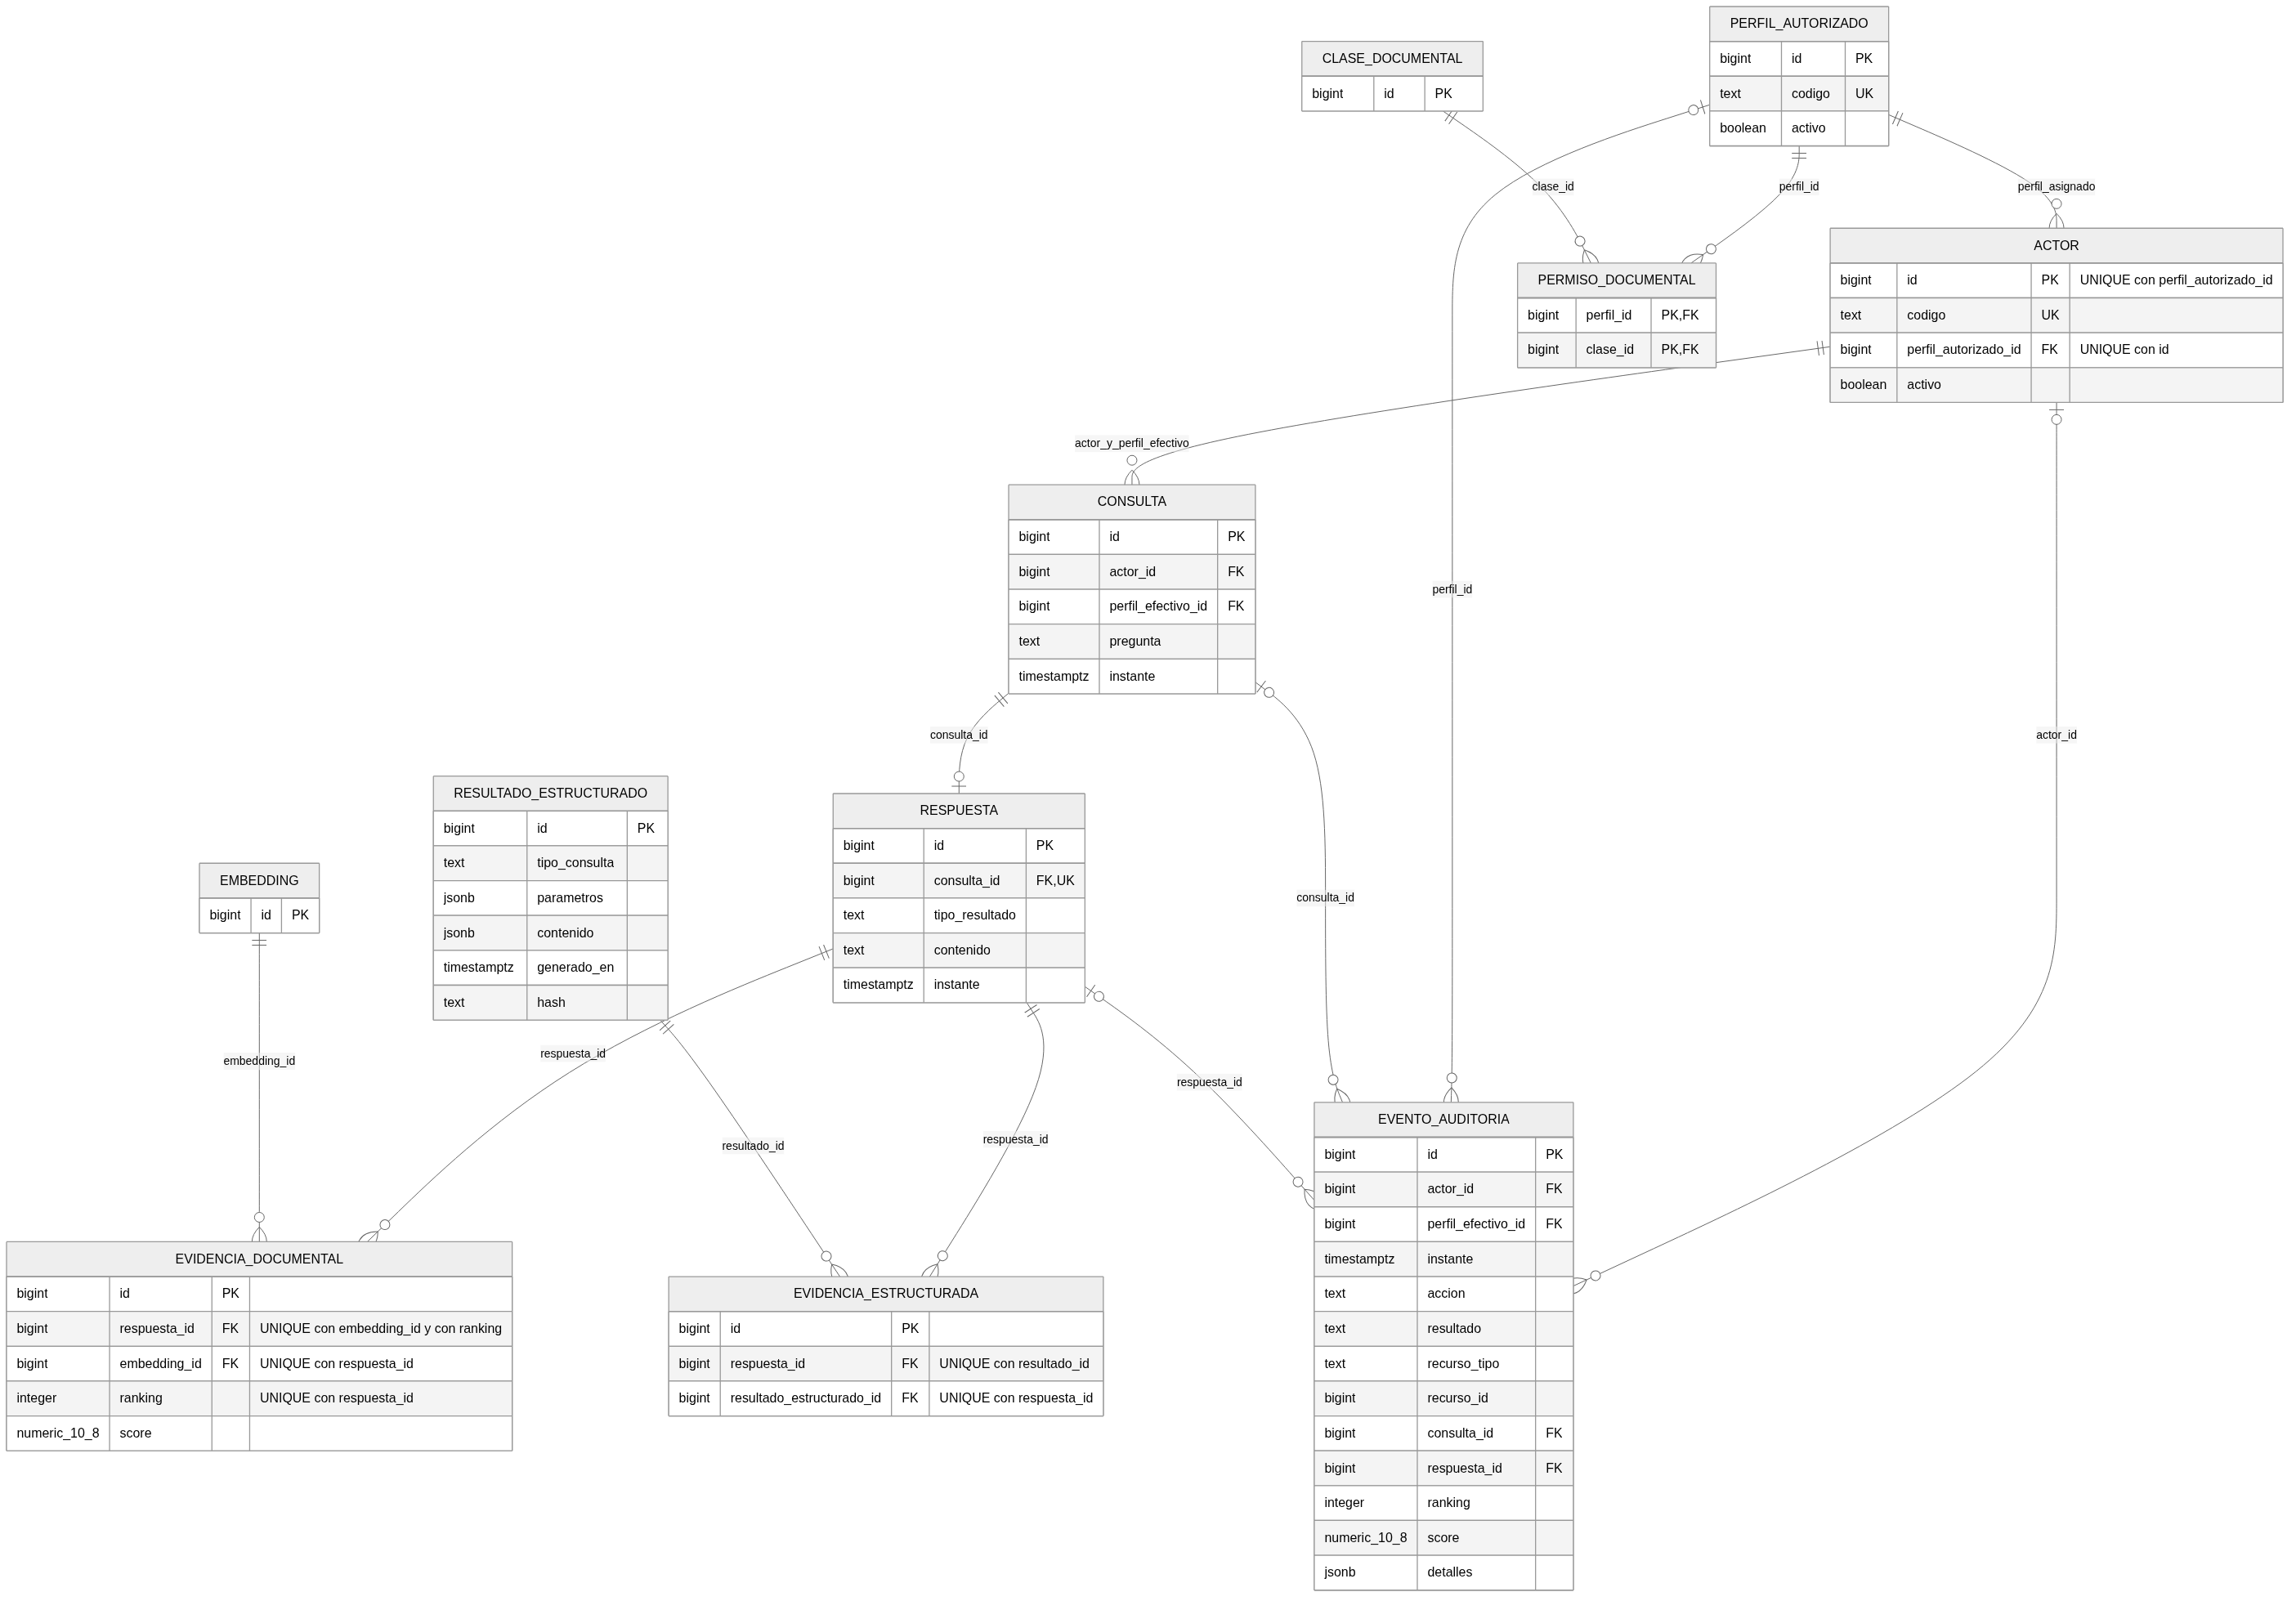
\includegraphics[width=0.85\linewidth]{fisico_seguridad.png}
\caption{Autorización, evidencia y auditoría en PostgreSQL.}
\label{fig:fisico-seguridad}
\end{figure}
\end{landscape}
\FloatBarrier

\begin{table}[htbp]
\centering
\small
\begin{tabularx}{\textwidth}{@{}lYY@{}}
\toprule
Decisión & Implementación & Propósito \\
\midrule
Identidad y tiempo & \texttt{BIGINT IDENTITY} y \texttt{TIMESTAMPTZ} &
Identificar filas y comparar vigencias sin depender de la zona horaria. \\
Metadatos variables & \texttt{JSONB} &
Conservar atributos heterogéneos sin trasladar el núcleo relacional a un
modelo documental. \\
Vectores & \texttt{VECTOR(32)} e índice HNSW con distancia coseno &
Ejecutar la prueba de recuperación top-k con vectores sintéticos y
reproducibles. \\
Integridad & \texttt{CHECK}, claves foráneas, \texttt{UNIQUE},
\texttt{EXCLUDE} y triggers diferidos &
Controlar estados, referencias, vigencias sin solape y reglas que abarcan
varias filas. \\
Acceso y trazabilidad & Roles, privilegios, RLS y triggers de auditoría &
Aplicar permisos antes del ranking y registrar operaciones sin permitir que el
rol de ejecución altere el historial. \\
\bottomrule
\end{tabularx}
\caption{Principales decisiones del modelo físico.}
\label{tab:decisiones-fisicas}
\end{table}
\FloatBarrier

Los índices B-tree cubren claves foráneas, filtros y joins usados por las
consultas. HNSW cubre el acceso vectorial. Los intervalos semiabiertos y
\texttt{EXCLUDE USING gist} impiden solapamientos en condiciones comerciales y
versiones publicadas. Los constraint triggers diferidos validan al cerrar la
transacción las reglas que abarcan varias filas.
